%
%

%%-----------------------------------------------------
%%-----------------------------------------------------
\section{Ofusca, que algo queda}

%%-----------------------------------------------------
\begin{frame}[fragile]
\frametitle{No todo el código se escribe para que sea legible...}

Este programa escribe ``3.141'' calculando Pi a partir de su propia área.

{\tiny
\begin{verbatim}
#define _ -F<00||--F-OO--;
int F=00,OO=00;main(){F_OO();printf("%1.3f\n",4.*-F/OO/OO);}F_OO()
{
            _-_-_-_
       _-_-_-_-_-_-_-_-_
    _-_-_-_-_-_-_-_-_-_-_-_
  _-_-_-_-_-_-_-_-_-_-_-_-_-_
 _-_-_-_-_-_-_-_-_-_-_-_-_-_-_
 _-_-_-_-_-_-_-_-_-_-_-_-_-_-_
_-_-_-_-_-_-_-_-_-_-_-_-_-_-_-_
_-_-_-_-_-_-_-_-_-_-_-_-_-_-_-_
_-_-_-_-_-_-_-_-_-_-_-_-_-_-_-_
_-_-_-_-_-_-_-_-_-_-_-_-_-_-_-_
 _-_-_-_-_-_-_-_-_-_-_-_-_-_-_
 _-_-_-_-_-_-_-_-_-_-_-_-_-_-_
  _-_-_-_-_-_-_-_-_-_-_-_-_-_
    _-_-_-_-_-_-_-_-_-_-_-_
        _-_-_-_-_-_-_-_
            _-_-_-_
}
\end{verbatim}
}

\begin{flushright}
{\small
\url{http://www0.us.ioccc.org/years-spoiler.html#1988_westley}
}
\end{flushright}

\end{frame}

%%-----------------------------------------------------
\begin{frame}[fragile]
\frametitle{The International Obfuscated C Code Contest}

\begin{columns}[T]
\begin{column}{.63\textwidth}
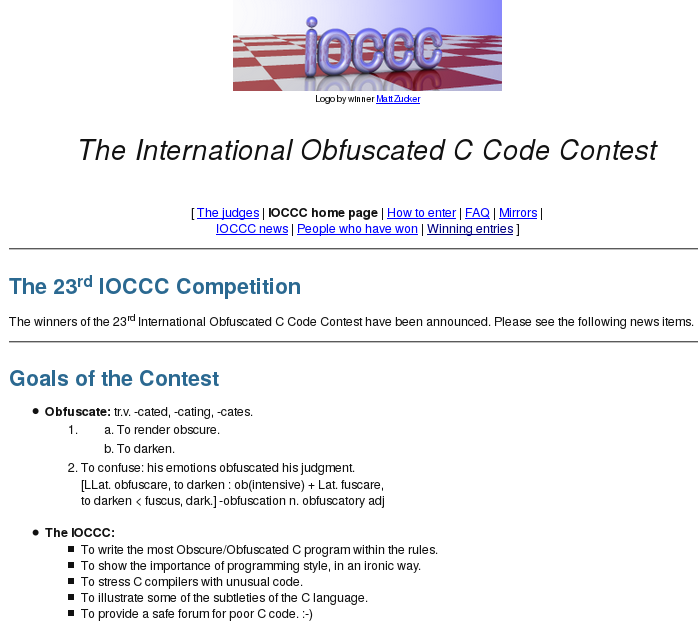
\includegraphics[width=8cm]{figs/obfuscated-ioccc}
\end{column}%
\hfill%
\begin{column}{.36\textwidth}
\begin{itemize}
\item Desde 1984
\item Celebrando la opacidad sintáctica \\
  (del lenguaje C)
\item \url{http://www.ioccc.org/}
\item Ganadores de cada concurso disponbiles
\end{itemize}
\end{column}%
\end{columns}


\begin{flushright}
{\footnotesize
\url{http://en.wikipedia.org/wiki/International_Obfuscated_C_Code_Contest}
}
\end{flushright}
\end{frame}

%%-----------------------------------------------------
\begin{frame}[fragile]
\frametitle{No sólo C, no sólo ofuscado (y también C y ofuscado)}

\begin{itemize}
\item Obfuscated Perl Contest \\
  Pero Perl es ruido de línea, ya sin ofuscar, ¿no?
\item Underhanded C Contest \\
  Código malicioso, pero que pasar un análisis riguroso
\item Weirdest obfuscated ``Hello World!'' \\
  StackExchange, ejemplos en varios lenguajes
\item IOCCC Flight Simulator \\
  ¡No me digas que no es maravilloso!
\end{itemize}

\begin{flushright}
{\small
\url{http://en.wikipedia.org/wiki/Obfuscated_Perl_Contest} \\
\url{http://www.underhanded-c.org/} \\
\url{http://codegolf.stackexchange.com/questions/22533/weirdest-obfuscated-hello-world} \\
\url{http://blog.aerojockey.com/post/iocccsim} \\
}
\end{flushright}
\end{frame}

%%-----------------------------------------------------
\begin{frame}
\frametitle{Mención aparte: Whitespace Programming Language}

\begin{center}
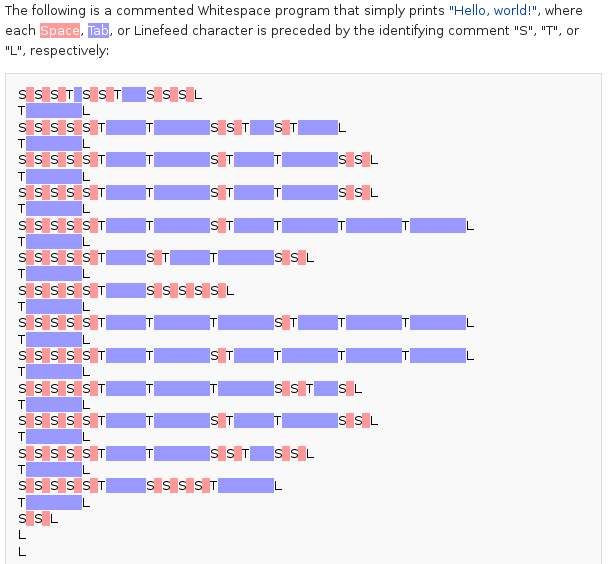
\includegraphics[width=7cm]{figs/obfuscated-whitespace}
\end{center}

\begin{flushright}
{\footnotesize
\url{http://compsoc.dur.ac.uk/whitespace/} \\
\url{http://en.wikipedia.org/wiki/Whitespace_\%28programming_language\%29}
}
\end{flushright}

\end{frame}

